\documentclass[tikz,border=10pt]{standalone}
\usepackage{amsmath}
\usetikzlibrary{shapes.geometric, arrows.meta, positioning}

\begin{document}
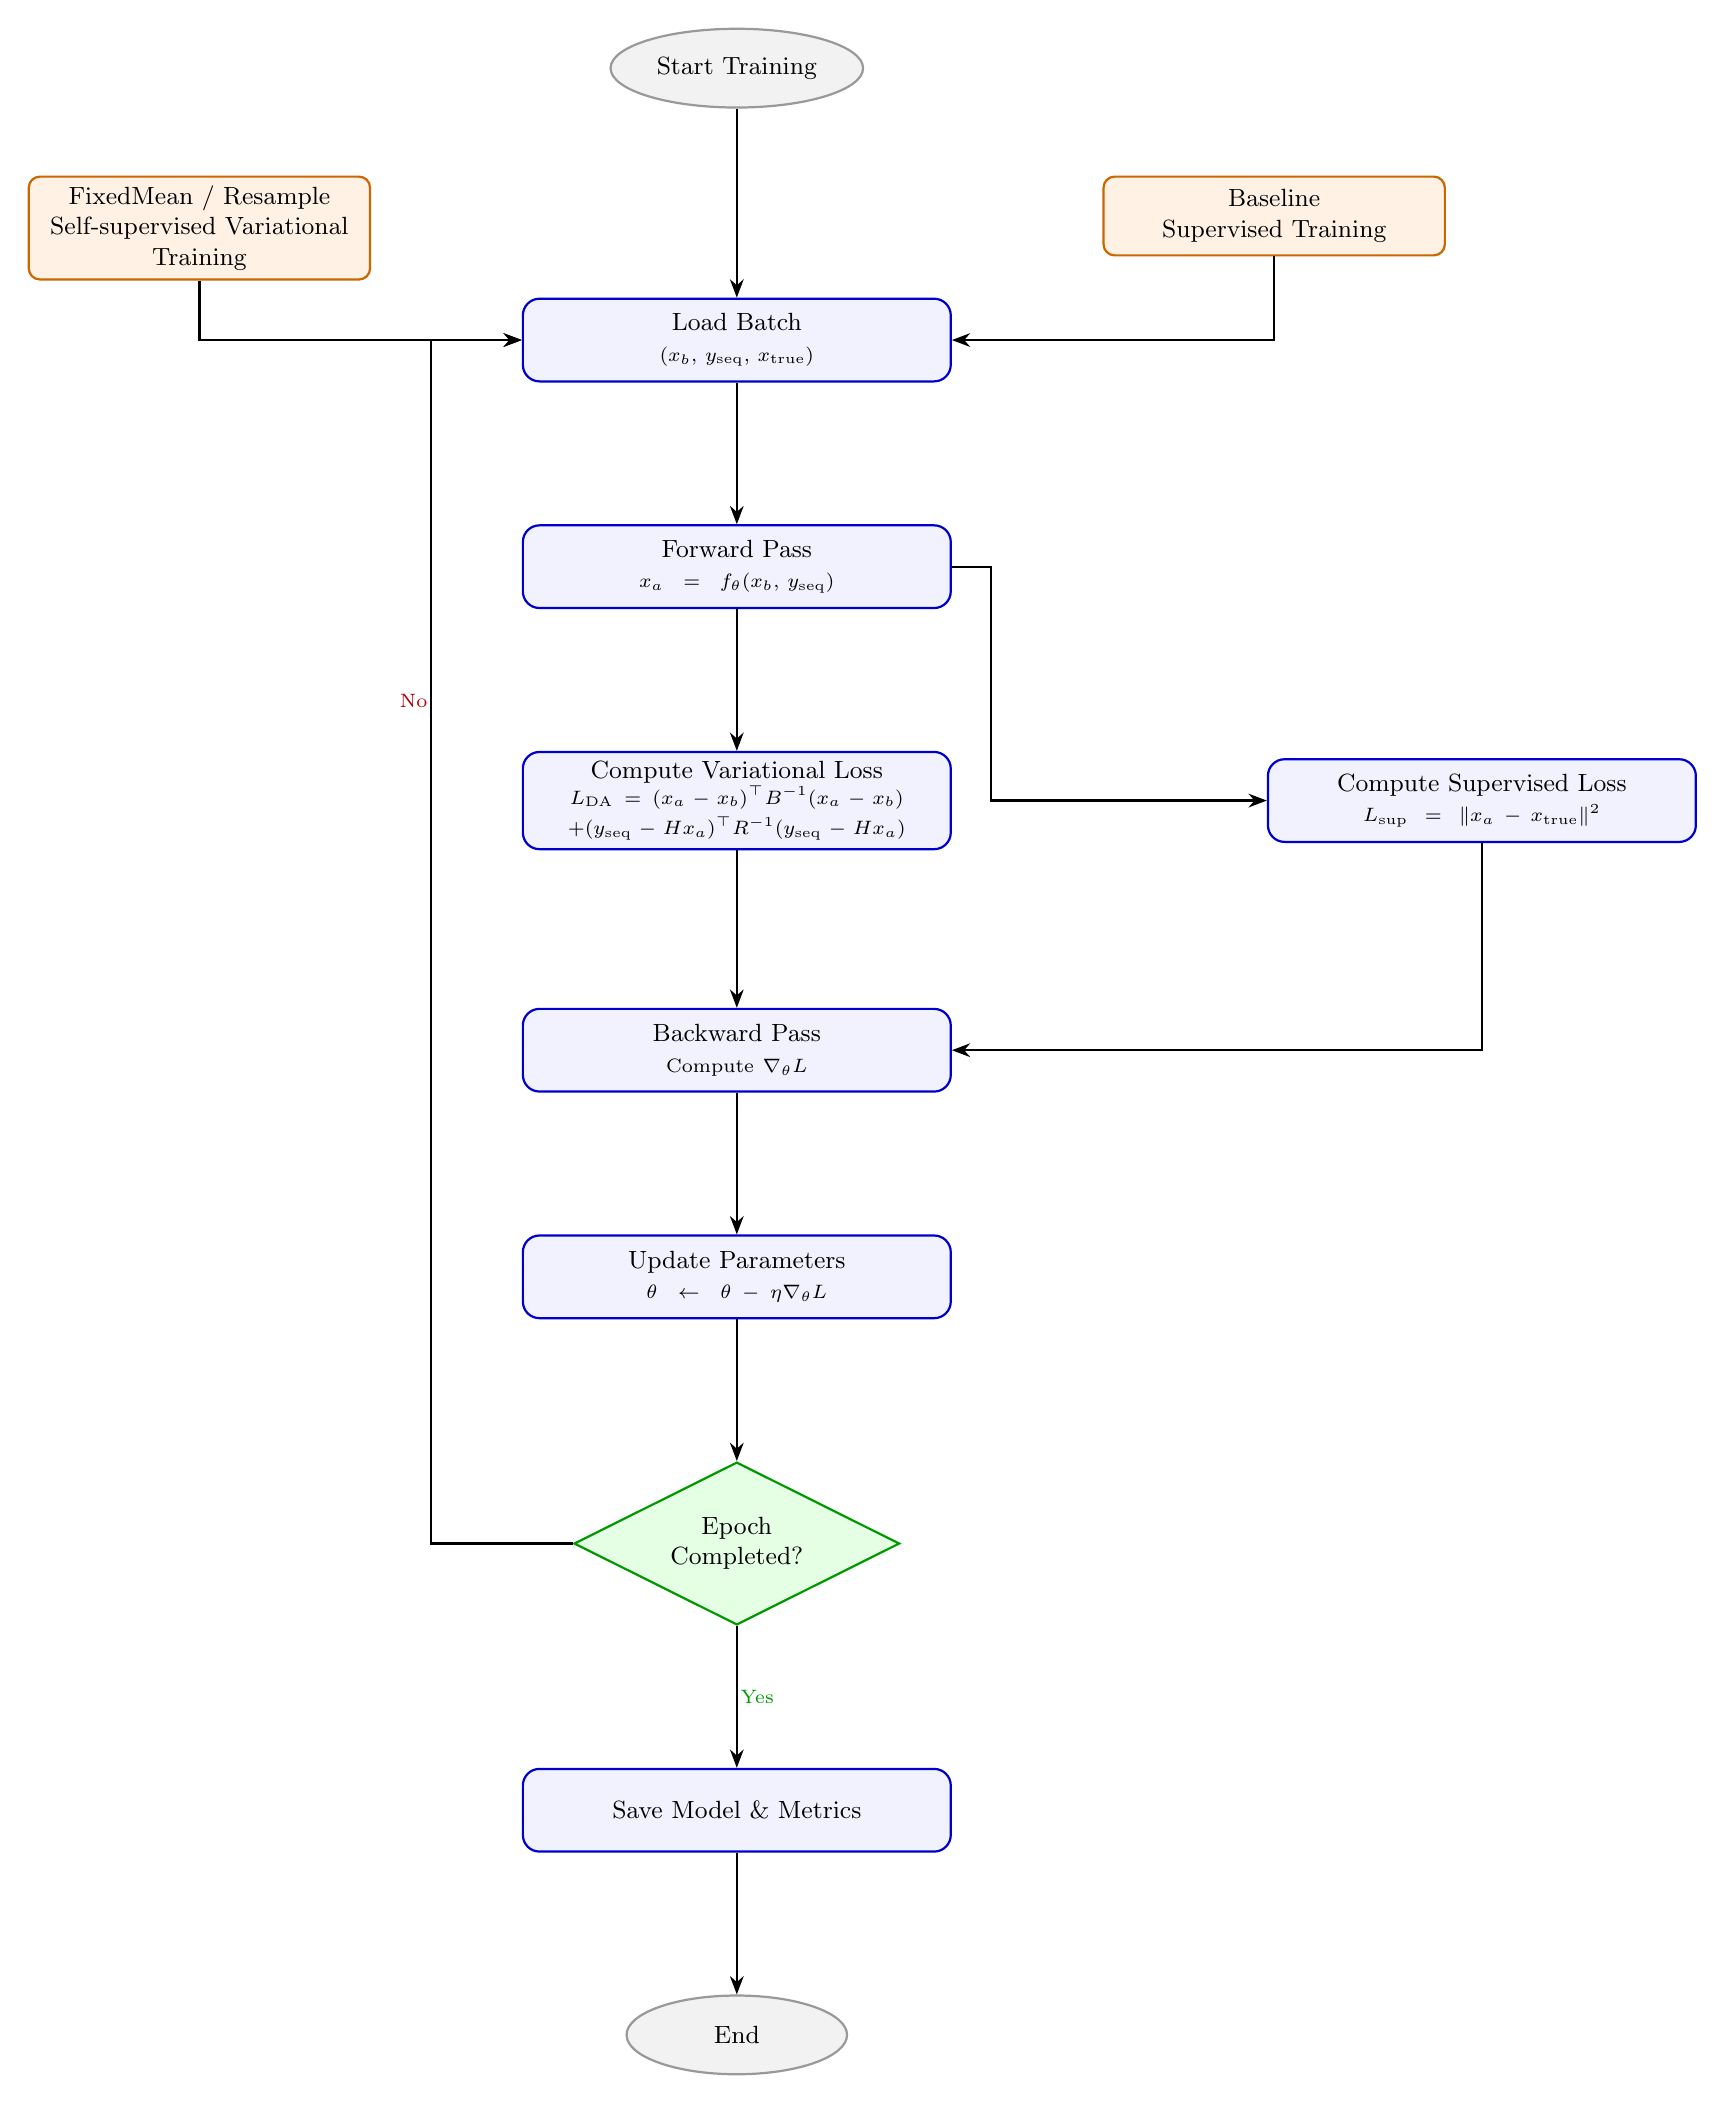
\begin{tikzpicture}[
  node distance=1.8cm and 2cm,
  >=Stealth,
  every node/.style={font=\small},
  io/.style={ellipse, draw=gray!80, fill=gray!10, thick,
             minimum width=2.8cm, minimum height=1cm, align=center},
  regime/.style={rectangle, draw=orange!80!black, fill=orange!10, thick,
             rounded corners=4pt, text width=4.1cm, align=center, minimum height=1cm},
  process/.style={rectangle, draw=blue!80!black, fill=blue!5, thick,
             rounded corners=6pt, text width=5.2cm, align=center, minimum height=1.05cm},
  decision/.style={diamond, draw=green!60!black, fill=green!10, thick,
             aspect=2, align=center, inner xsep=1mm, inner ysep=1mm, text width=2.2cm},
  arrow/.style={-Stealth, thick},
  lab/.style={font=\scriptsize, inner sep=1pt}
]

% Main flow
\node[io] (start) {Start Training};

\node[regime, below left=1cm and 3.5cm of start] (selfsup)
  {FixedMean / Resample\\Self-supervised Variational\\Training};
\node[regime, below right=1cm and 3.5cm of start] (sup)
  {Baseline\\Supervised Training};

\node[process, below=2.4cm of start] (load)
  {Load Batch\\{\scriptsize $(x_b,\, y_{\text{seq}},\, x_{\text{true}})$}};
\node[process, below=1.8cm of load] (forward)
  {Forward Pass\\{\scriptsize $x_a=f_\theta(x_b,\, y_{\text{seq}})$}};
\node[process, below=1.8cm of forward] (varloss)
  {Compute Variational Loss\\{\scriptsize
  $L_{\text{DA}}=(x_a-x_b)^\top B^{-1}(x_a-x_b)$\\
  $+(y_{\text{seq}}-Hx_a)^\top R^{-1}(y_{\text{seq}}-Hx_a)$}};
\node[process, right=4cm of varloss] (suploss)
  {Compute Supervised Loss\\{\scriptsize $L_{\text{sup}}=\lVert x_a-x_{\text{true}}\rVert^2$}};
\node[process, below=2.0cm of varloss] (backward)
  {Backward Pass\\{\scriptsize Compute $\nabla_\theta L$}};
\node[process, below=1.8cm of backward] (update)
  {Update Parameters\\{\scriptsize $\theta \leftarrow \theta - \eta \nabla_\theta L$}};
\node[decision, below=1.8cm of update] (epoch)
  {Epoch\\Completed?};
\node[process, below=1.8cm of epoch] (save)
  {Save Model \& Metrics};
\node[io, below=1.8cm of save] (end)
  {End};

% Arrows
\draw[arrow] (start.south) -- (load.north);
\draw[arrow] (selfsup.south) |- (load.west);
\draw[arrow] (sup.south) |- (load.east);
\draw[arrow] (load.south) -- (forward.north);
\draw[arrow] (forward.south) -- (varloss.north);
\draw[arrow] (varloss.south) -- (backward.north);
\draw[arrow] (backward.south) -- (update.north);
\draw[arrow] (update.south) -- (epoch.north);
\draw[arrow] (epoch.south) -- node[lab, right, text=green!60!black] {Yes} (save.north);
\draw[arrow] (save.south) -- (end.north);

% Connect supervised loss horizontally
\draw[arrow] (forward.east) --++(5mm,0) |- (suploss.west);
\draw[arrow] (suploss.south) |- (backward.east);

% No-loop back to Load
\draw[arrow] (epoch.west) --++(-18mm,0) |- node[lab, left, text=red!70!black, pos=0.35]{No} (load.west);

\end{tikzpicture}
\end{document}
